\documentclass[a4j,twocolumn]{jsarticle}
\usepackage{amssymb} % 高度な数式を表記するために使用
\usepackage[dvipdfmx]{graphicx}		% 図を入れるときに使用
\usepackage{wrapfig}		% 図の周りに本文を流し込みたいときに使用
\usepackage{here}
\usepackage{subfigure}

\def\Vec#1{\mbox{\boldmath $#1$}}
\usepackage[dvipdfmx]{graphics}

\setlength{\textheight}{275mm}
\headheight 5mm
\topmargin -30mm
\textwidth 185mm
\oddsidemargin -15mm
\evensidemargin -15mm
\pagestyle{empty}

\begin{document}
\vskip 1.5em%

\title{三面図を利用した粒界原子配列の表示}
\author{関西学院大学 情報科学科 西谷研究室 1549 成田大樹}
\date{}
\maketitle

\section{序論}
本研究の目的は,原子間ポテンシャルを用いたシミュレーションの結果と大槻による実験結果の矛盾を解明することである.
両者の具体的な相違点は,小傾角粒界エネルギーの0度,及び90度における立ち上がりの傾き方である.原子間ポテンシャルを用いたシミュレーションの結果では,傾きが異なっていたのに対し,大槻の実験結果では,傾きが左右対称になっていた.

この矛盾を解明するために,西谷研究室では様々な手法をこれまで試してきた.
岩佐の研究では,最安定な原子配置を探索するために原子の削除操作を取り入れ,
第一原理計算ソフトVASPを用いて構造緩和し,系全体のエネルギーを計算した.
その結果,小傾角粒界エネルギーが大槻の結果を再現する程度の低いエネルギーを得ることができた.ところが,粒界がより低い角度になった状態を計算していたため,構造緩和に過ちが生じていた\cite{Iwasa}.
これは,安定構造の原子配列を視覚的に確認をしなかったことが原因である.
この失敗を踏まえて,原子配列を容易に視覚化できるためのソフトを本研究で開発する.

\section{ソフト開発の手法}
本研究で開発するソフトは,MVCモデルで作成し,原子配列を2次元で描画する.
MVCモデルは,三要素で構成されており,各機能が直交化されているため,作業の分業化がしやすい\cite{MVC}.したがって,原子配列の結果を画面表示する機能構築に特化した開発が取り組める.
原子配列の出力は,原子座標を格納したPOSCAR形式のファイルを読み込んで,SVG形式で表示する.また.原子配列を三方向から投影した三面図で描画する.
これまでの原子配列の構造は,結晶構造描画ソフトVESTAを用いて3次元表示で確認してきた.三面図で表示することにより,図\ref{fig:one}のように,各面から原子の配置を直感的かつ簡易に確認できるようになる.なお,三面図の構成には規定があり,図面の各配置を遵守して描画しなければらない\cite{ThreeViewDrawing}.

\begin{figure}[h]
\begin{center}
   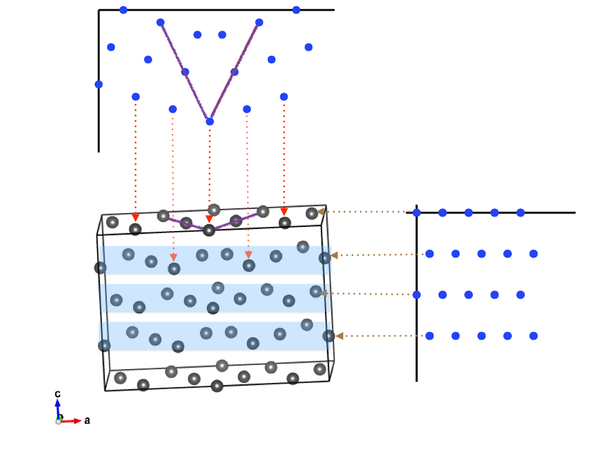
\includegraphics[width=55mm]{vesta_two_dimension.jpeg} 
     \caption{VESTAの投影図を2次元化した図.}
  \label{fig:one}
\end{center}
\end{figure}

\section{原子配列の表示結果}
ソフト開発をおこなう中で,様々な用途に合わせて原子配列を表示することが可能になった.まず,削除操作をおこなった原子配列の表示では,図\ref{fig:two}(a)のように,削除の有無によって原子の色と大きさを変える描画をした.その結果,削除された原子の個数,並びに各位置を視覚的に把握することができた.また,図\ref{fig:two}(b)のように,構造緩和による原子の移動を三面図で表示した.これにより,原子が移動した経路,並びに構造緩和に過ちが生じていないかを容易に確認することができるようになったなった. さらに,上面から見た各層の原子の位置を正確に把握するために,指定したz軸の層の原子を白抜きする機能をソフトに追加した.

\begin{figure}[h]
\begin{center}
\begin{tabular}{cc}
   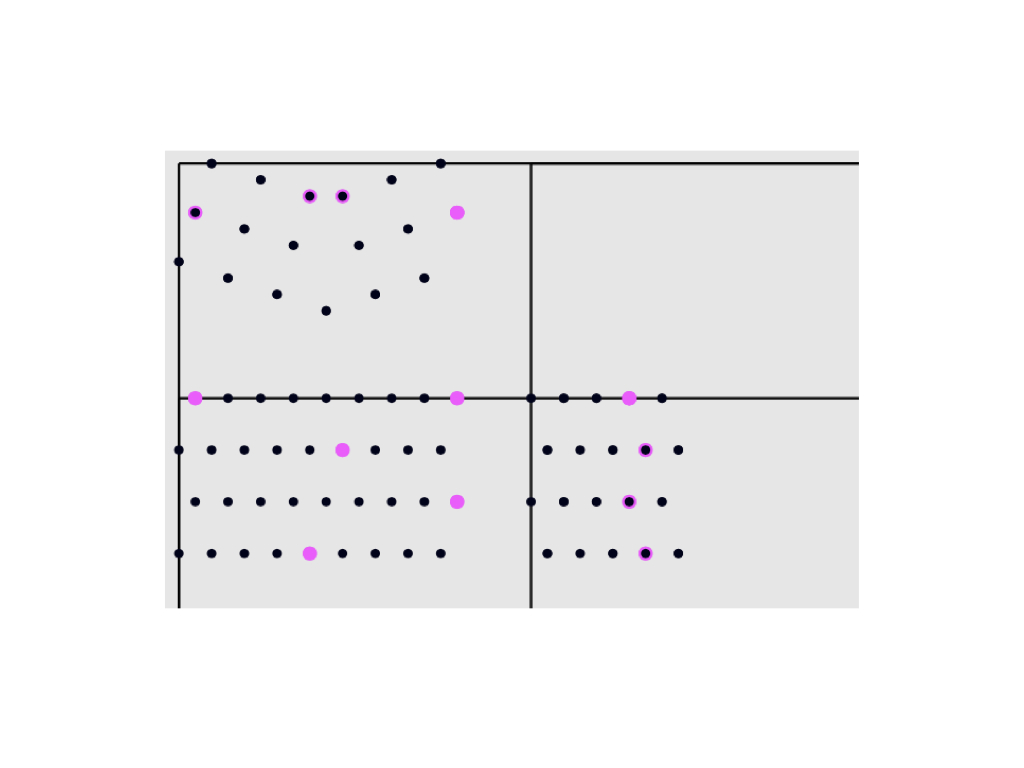
\includegraphics[width=48mm]{deleted_atoms.jpg} &
   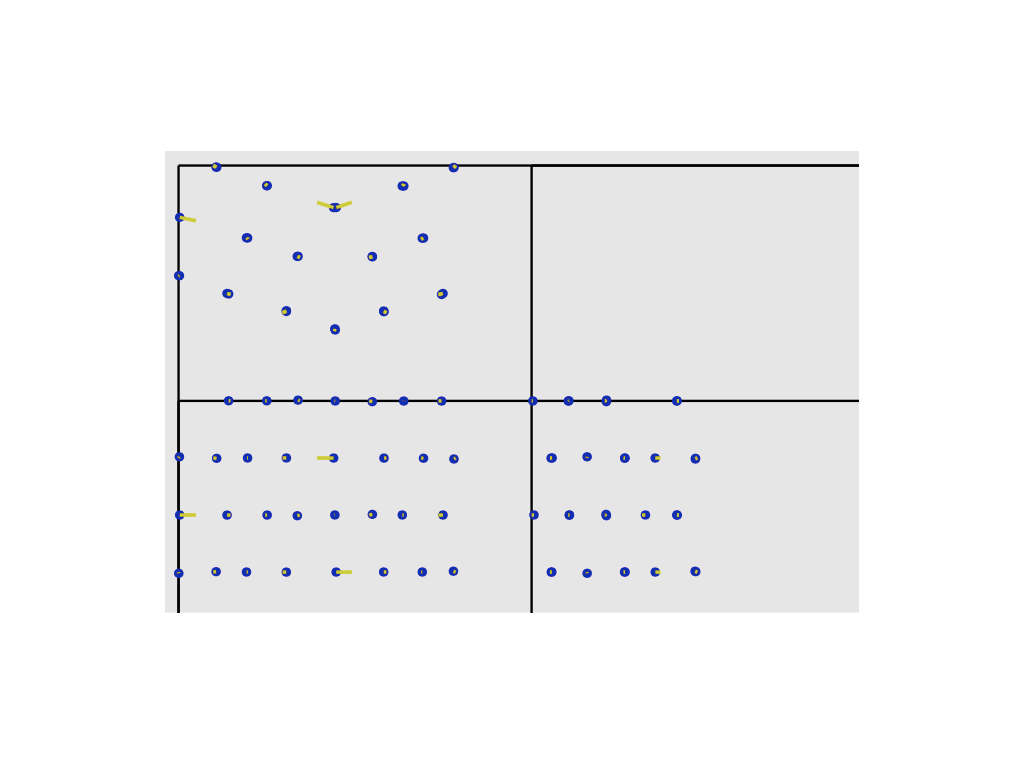
\includegraphics[width=48mm]{change_position.jpg} \\
   (a) & (b)
\end{tabular}
  \caption{(a) 削除した原子の識別表示と(b)構造緩和による原子移動を表した三面図.}
  \label{fig:two}
\end{center}
\end{figure}

\section{総括}
三面図を用いて原子配列を表示したことにより,削除操作,及び構造緩和をおこなった際の原子配置を視覚化することができた.また,構造緩和をおこなう際に使用したPOSCARファイルに過ちがあったことに気づいた.これは,今までの原子配列が結晶構造描画ソフト"VESTA"による3次元表示であり,原子の細かい位置が確認できず,原子が不足していることを認識できなかったためである.したがって,粒界原子配列の構造緩和をおこなう計算を見直す必要がある.

\begin{thebibliography}{9}
\bibitem{Iwasa} 原子削除操作を加えた対称傾角粒界のエネルギー計算, 岩佐恭佑 (関西学院大学 理工学部研究科情報科 学士論文 2016).. 
\bibitem{MVC}   MVCのベストプラクティス, Yii Supporters, yiiframework, \verb|http://www.yiiframework.com/doc/guide/1.1/ja/basics.best-practices,| 2017/2/11アクセス.
\bibitem{ThreeViewDrawing}   三面図(機械設計のための基礎製図), 独立行政法人 海上技術安全研究所, NMRI, \verb|https://www.nmri.go.jp/eng/khirata/mechdesign/ch04/ch04.html,| 2017/2/11アクセス.
\end{thebibliography}

\end{document}
